\documentclass{ctexart}
\usepackage{amsmath,bm}
\usepackage{setspace}
\usepackage{xeCJK}
\usepackage{indentfirst}
\usepackage{listings}
\usepackage{graphicx}
\usepackage{subfigure}
\usepackage{amsfonts,amssymb}
\usepackage[a4paper,scale=0.8]{geometry}
\usepackage{hyperref}
\usepackage{pythonhighlight}
\usepackage{float}
\setCJKmainfont{华光书宋_CNKI}
\newCJKfontfamily\kaiti{华光楷体_CNKI}
\newCJKfontfamily\hei{华光黑体_CNKI}
\newCJKfontfamily\fsong{华光仿宋_CNKI}
\newfontfamily\code{Courier New}
\linespread{1.5} \setlength\parindent{2 em}
\title{\Huge 中国科学技术大学计算机学院\\《人工智能基础》实验报告}
\date{\LARGE 2021.05.28}
\begin{document}
\begin{hei}  \maketitle\end{hei}
\begin{figure}[htbp]	
	\centering	
	
\includegraphics[scale=0.4]{USTC.png}
		
\end{figure}
\begin{LARGE}\begin{align*}&\text{实验题目:\underline{Search和Multiagent}}\\ 
	&\text{学生姓名:\underline{胡毅翔}}\\
	&\text{学生学号:\underline{PB18000290}}\end{align*}\end{LARGE}
 \par 
 \par\par
\centerline{\large 计算机实验教学中心制}
\par \centerline {\large 2019年9月}
\newpage
\section{\hei 实验目的}
1.实现BFS算法和A*算法。
\par2.实现minimax算法和alpha-beta算法。
\section{\hei 实验环境}
1.PC一台。\par
2.Windows 10操作系统。\par
3.Git Bash\par
4.Python 3.8.1
\section{\hei 算法思路}
\subsection{\hei BFS算法}
BFS(Breadth-first search)算法,即广度优先搜索算法。其边界选用的是FIFO队列。其完备性已在课堂中得到证明。
在本次实验中,每一步的代价均相同,故满足最优性条件,一定返回最优解。设$b$为最大分支数,$d$为目标节点的最小深度。
算法的时间复杂度是$O\left(b^{d}\right)$,空间复杂度是$O\left(b^{d}\right)$。
\par 算法的伪代码如下:
\begin{figure}[htbp]	
	\centering	
	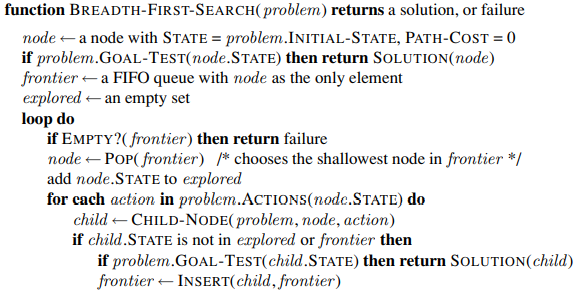
\includegraphics[scale=0.5]{BFS_w.png}
		
\end{figure}
\par 本次实验中实现的\textbf{Python}代码如下:
\begin{python}
def myBreadthFirstSearch(problem):

    visited = {}
    frontier = util.Queue()

    frontier.push((problem.getStartState(), None))

    while not frontier.isEmpty():
        state, prev_state = frontier.pop()
        if problem.isGoalState(state):
            solution = [state]
            while prev_state != None:
                solution.append(prev_state)
                prev_state = visited[prev_state]
            return solution[::-1]
        if state not in visited:
            visited[state] = prev_state
            for next_state, step_cost in problem.getChildren(state):
                frontier.push((next_state, state))
    return []
	\end{python}
\subsection{\hei A*算法}
A*(A-star)算法,即A星算法。该算法的评估函数为:
$$f\left(n\right)=g\left(n\right)+h\left(n\right)$$\par
其中$f\left(n\right)$表示经过节点$n$的最低耗散的估计函数,$g\left(n\right)$
表示到达节点$n$的耗散,$h\left(n\right)$为启发函数,表示从节点$n$到目标节点的
最低耗散路径的耗散估计值。
\par 可采纳的启发式函数须满足:
$$h\left(n\right)\leq  h^{*}\left(n\right)$$\par
其中$h^{*}\left(n\right)$表示从节点$n$到目标节点的
最低耗散路径的实际耗散值。\par 
A*算法的最优性,完备性已在课堂上得到证明。其伪代码如下:
\begin{figure}[htbp]	
	\centering	
	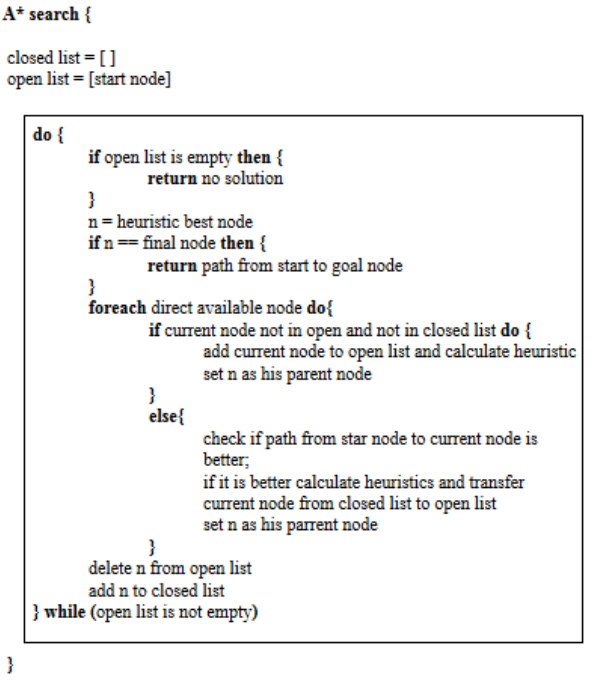
\includegraphics[scale=0.37]{astar.png}
		
\end{figure}
\par 本次实验中实现的\textbf{Python}代码如下:
\begin{python}
def myAStarSearch(problem, heuristic):

    visited = {}
    frontier = util.PriorityQueue()
    frontier.update((problem.getStartState(), None, 0),
                    heuristic(problem.getStartState()))

    while not frontier.isEmpty():
        state, prev_state, cost = frontier.pop()
        if problem.isGoalState(state):
            solution = [state]
            while prev_state != None:
                solution.append(prev_state)
                prev_state = visited[prev_state]
            return solution[::-1]
        if state not in visited:
            visited[state] = prev_state
            for next_state, step_cost in problem.getChildren(state):
                h_n = heuristic(next_state)
                frontier.update(
                    (next_state, state, cost+step_cost), cost+step_cost+h_n)
    return []
\end{python}
\subsection{\hei minimax算法}
minimax算法,即极小极大值算法。该算法在假设对手也是用最优策略的条件下。
能导致至少不必其他策略车的结果。换句话说,假设两个游戏者都按照最优策略进行,那么节点的极小极大值就
是对应状态的效用值。
\begin{figure}[htbp]	
	\centering	
	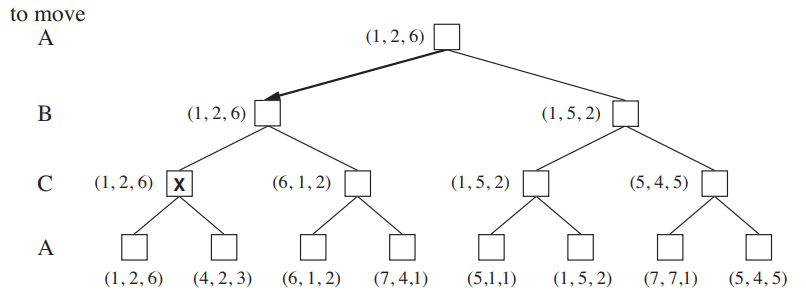
\includegraphics[scale=0.55]{mm.png}
		
\end{figure}
\par
其算法的完备性,最优性已在课堂中得到证明。设$b$为最大分支数,$m$为搜索树的最大深度。
算法的时间复杂度是$O\left(b^{m}\right)$,空间复杂度是$O\left(bm\right)$。
\par 算法的伪代码如下:
\begin{figure}[htbp]	
	\centering	
	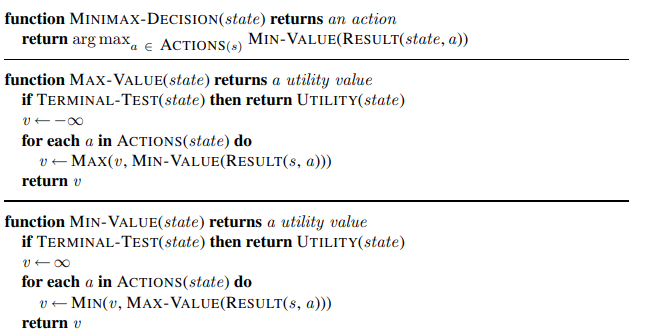
\includegraphics[scale=0.45]{minimax.png}
		
\end{figure}
\par 本次实验中实现的\textbf{Python}代码如下:
\begin{python}
class MyMinimaxAgent():

    def __init__(self, depth):
        self.depth = depth

    def minimax(self, state, depth):
        if state.isTerminated():
            return None, state.evaluateScore()

        best_state, best_score = None, - \
            float('inf') if state.isMe() else float('inf')

        for child in state.getChildren():
            if state.isMe():
                _, tmp_score = self.minimax(child, depth-1)
                if tmp_score > best_score:
                    best_score = tmp_score
                    best_state = child
            else:
                if child.isMe() and depth == 0:
                    tmp_score = child.evaluateScore()
                    if tmp_score < best_score:
                        best_score = tmp_score
                        best_state = child
                else:
                    _, tmp_score = self.minimax(child, depth)
                    if tmp_score < best_score:
                        best_score = tmp_score
                        best_state = child
        return best_state, best_score

    def getNextState(self, state):
        best_state, _ = self.minimax(state, self.depth)
        return best_state
	\end{python}
\subsection{\hei alpha-beta算法}
alpha-beta算法的思路与minimax算法类似,增加了$\alpha$,$\beta$两个参数。$\alpha$表示
到目前为止在路径上的任意点发现的$MAX$的最佳选择。$\beta$则表示
到目前为止在路径上的任意点发现的$MIN$的最佳选择。通过与这两个参数进行比较来判断后续的搜索是否必要,减少计算量。
\par 这一剪枝操作不会改变minimax的最终结果。在最优情况下,可以把时间复杂度降至$O\left(b^{m/2}\right)$,但在最坏情况下不会获得性能提升。

\par 算法的伪代码如下:
\begin{figure}[H]	
	\centering	
	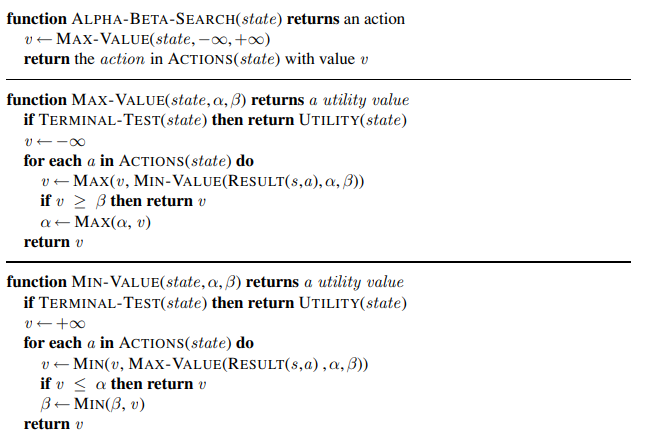
\includegraphics[scale=0.6]{alphabeta.png}
		
\end{figure}
\par 本次实验中实现的\textbf{Python}代码如下:
\begin{python}
class MyAlphaBetaAgent():

    def __init__(self, depth):
        self.depth = depth

    def alphabeta(self, state, depth, alpha, beta):
        if state.isTerminated():
            return None, state.evaluateScore()
        best_state, best_score = None, - \
            float('inf') if state.isMe() else float('inf')
        for child in state.getChildren():
            if state.isMe():
                _, tmp_score = self.alphabeta(child, depth-1, alpha, beta)
                if tmp_score > best_score:
                    best_score = tmp_score
                    best_state = child
                alpha = max(alpha, best_score)
                if best_score > beta:
                    return best_state, best_score
            else:
                if child.isMe() and depth == 0:
                    tmp_score = child.evaluateScore()
                else:
                    _, tmp_score = self.alphabeta(child, depth, alpha, beta)
                if tmp_score < best_score:
                    best_score = tmp_score
                    best_state = child
                beta = min(beta, best_score)
                if best_score < alpha:
                    return best_state, best_score
        return best_state, best_score

    def getNextState(self, state):
        best_state, _ = self.alphabeta(
            state, self.depth, float("-inf"), float("inf"))
        return best_state
	\end{python}
\section{实验结果}
\subsection{\hei BFS算法}
\begin{figure}[H]	
	\centering	
	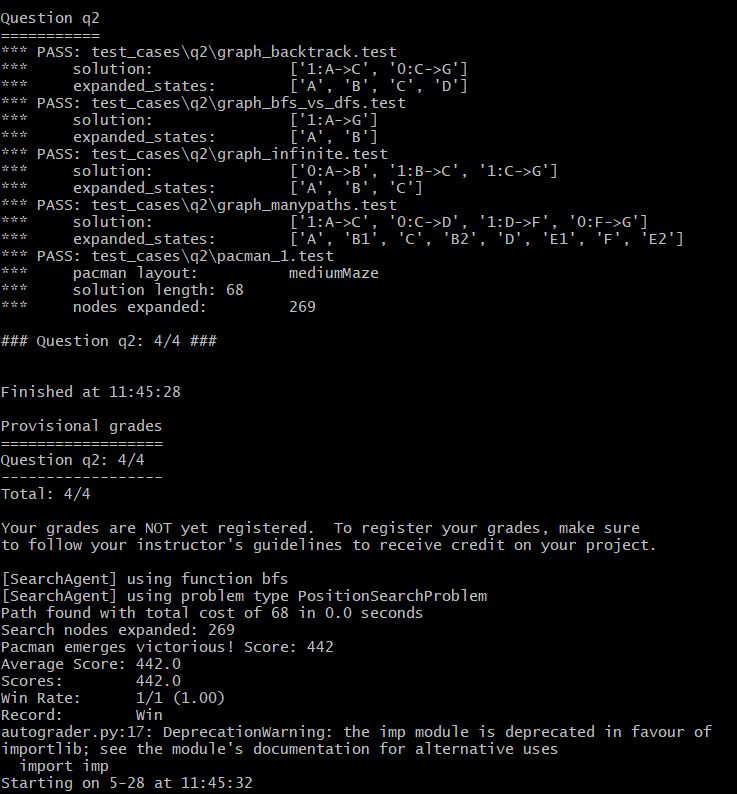
\includegraphics[scale=0.6]{bfs.png}
		
\end{figure}
\subsection{\hei A*算法}
\begin{figure}[H]	
	\centering	
	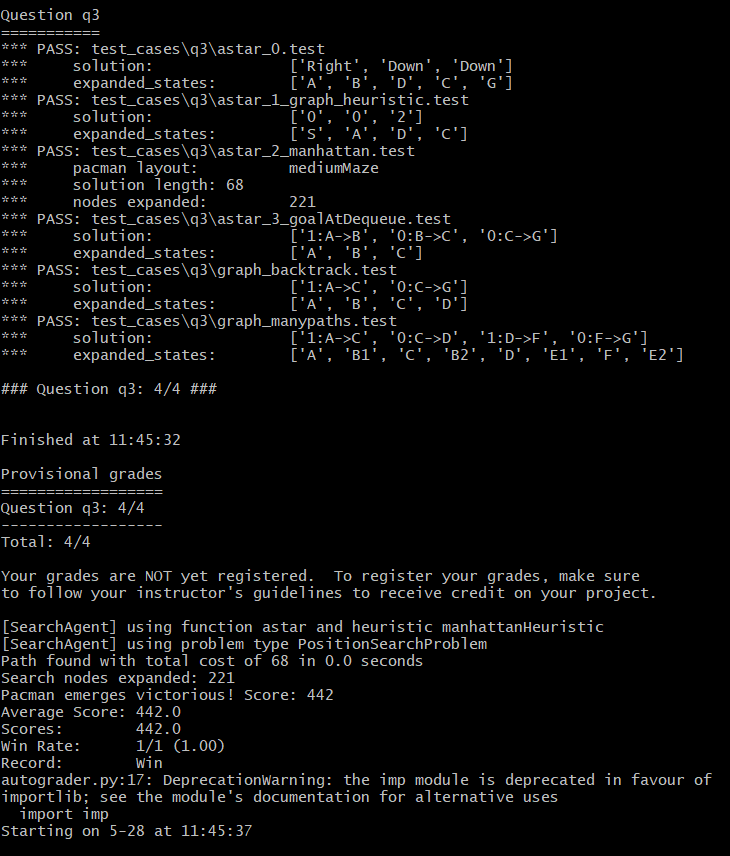
\includegraphics[scale=0.6]{ax.png}
		
\end{figure}
\subsection{\hei minimax算法}
\begin{figure}[H]	
	\centering	
	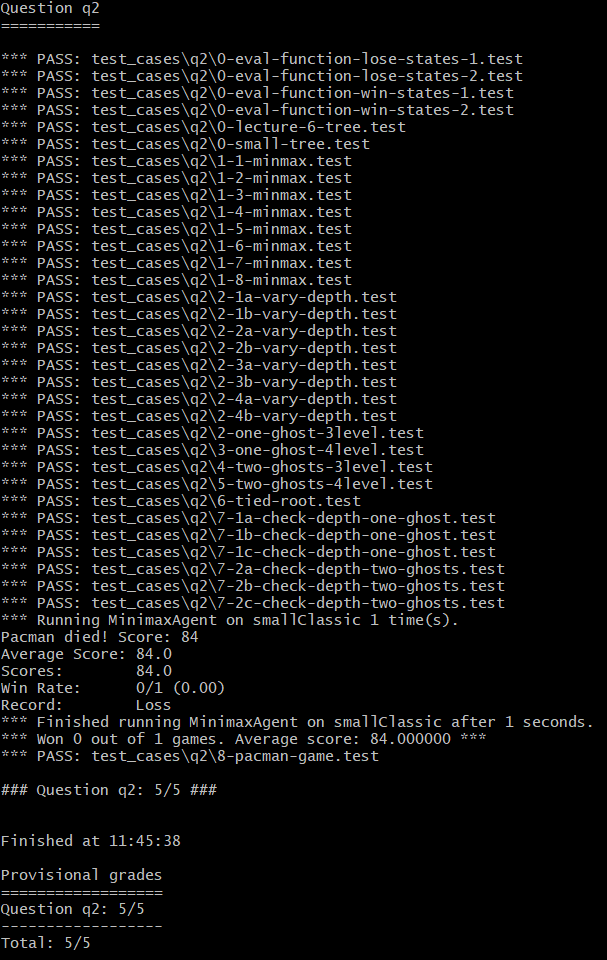
\includegraphics[scale=0.6]{mini.png}
		
\end{figure}
\subsection{\hei alpha-beta算法}
\begin{figure}[H]	
	\centering	
	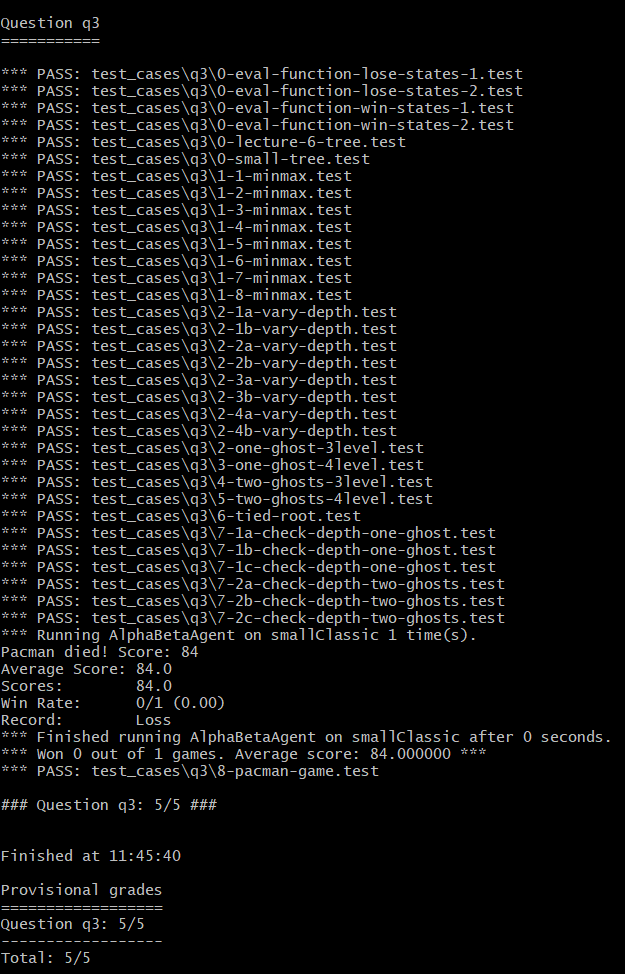
\includegraphics[scale=0.6]{ab.png}
		
\end{figure}
\section{\hei 总结}
本次实验实现了BFS,A*,minimax,alpha-beta四种算法,加深了对课堂所学知识的理解。通过吃豆人
游戏的方式,也增加了同学们对课程实验的兴趣。
\end{document}